\documentclass[UTF8]{ctexbeamer}
\usetheme{Madrid}
% \usecolortheme{beaver}
\usepackage{hyperref}
\usepackage{graphicx}
\usepackage{wrapfig}
\usepackage{caption}
\usepackage{subcaption}
\DeclareGraphicsExtensions{.eps,.ps,.jpg,.bmp,.png}


\title{Linux 个性化与建站体验}

\author{中国科学技术大学 LUG}

\date{March 29, 2020}

\AtBeginSection[]
{
	\begin{frame}
		\frametitle{Table of Contents}
		\tableofcontents[currentsection]
	\end{frame}
}



\begin{document}

\frame{\titlepage}
\begin{frame}
    % Table of contents 目录/大纲页
    % 自动实现对section的收集,并绘制成目录页
	\frametitle{Table of Contents}
	\tableofcontents
\end{frame}

\section{桌面系统}
\begin{frame}{桌面系统}
    早期几乎所有系统都是通过命令行管理的。
    
    \begin{columns}
        \column{0.2\textwidth}
        \begin{figure}
            \centering
            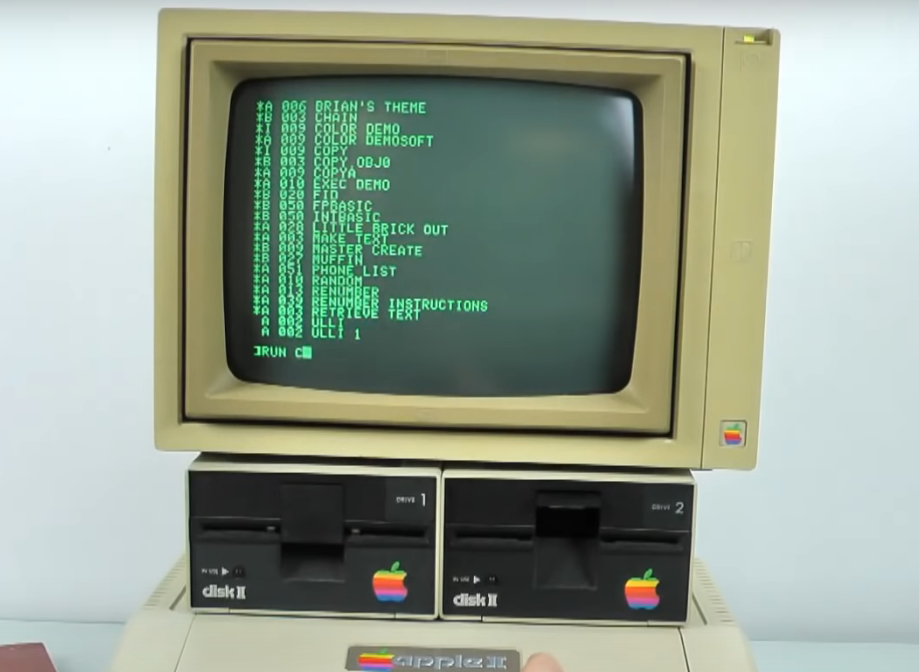
\includegraphics[width=\textwidth]{apple.png}
            \caption{Apple II}
            \label{fig:appleii}
        \end{figure}
        \column{0.2\textwidth}
        \begin{figure}
            \centering
            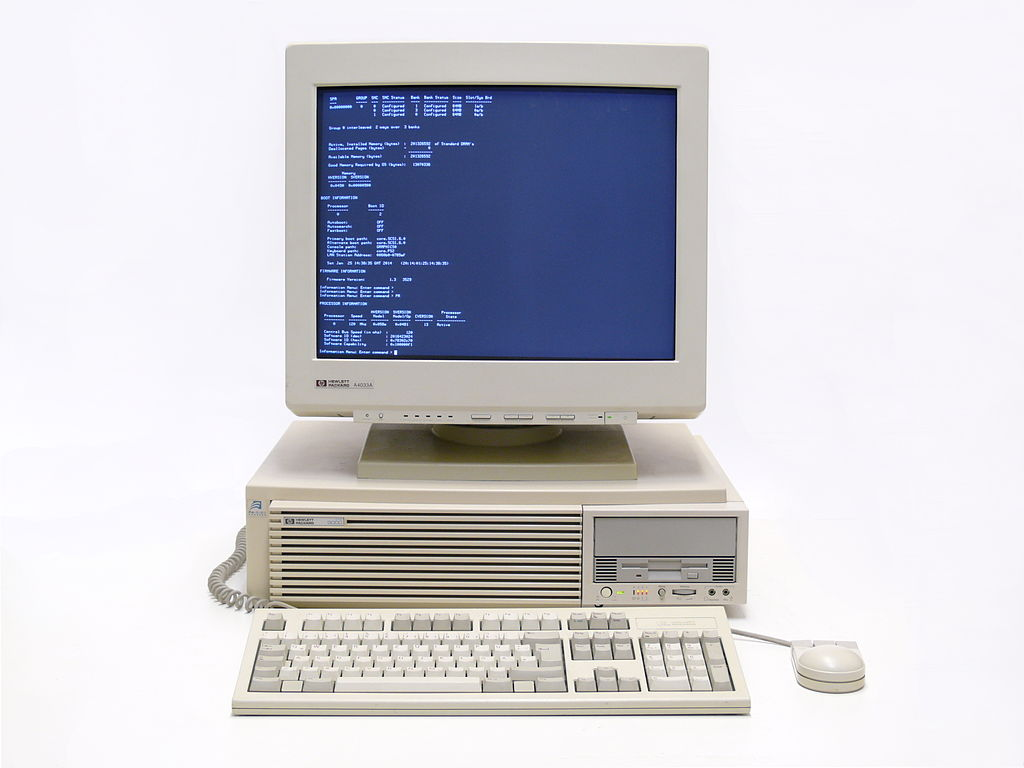
\includegraphics[width=\textwidth]{dell.png}
            \caption{Dell}
            \label{fig:dell}
        \end{figure}
        \column{0.3\textwidth}
        \begin{figure}
            \centering
            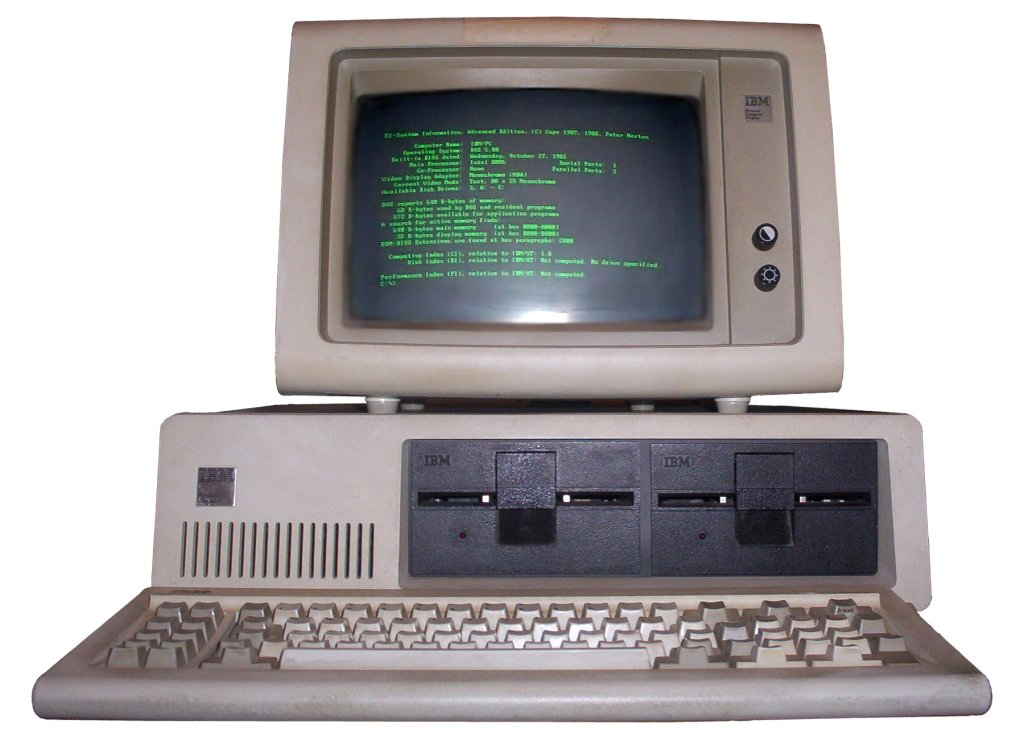
\includegraphics[width=\textwidth]{ibm-pc-5150.png}
            \caption{IBM PC 5150}
            \label{fig:ibmpc}
        \end{figure}
    \end{columns}
\end{frame}

\begin{frame}{桌面系统}
    随着时代的发展,人们不再满足于黑底白字的命令行界面,开发出来了图形环境。
    
    \begin{columns}
        \column{0.2\textwidth}
        \begin{figure}
            \centering
            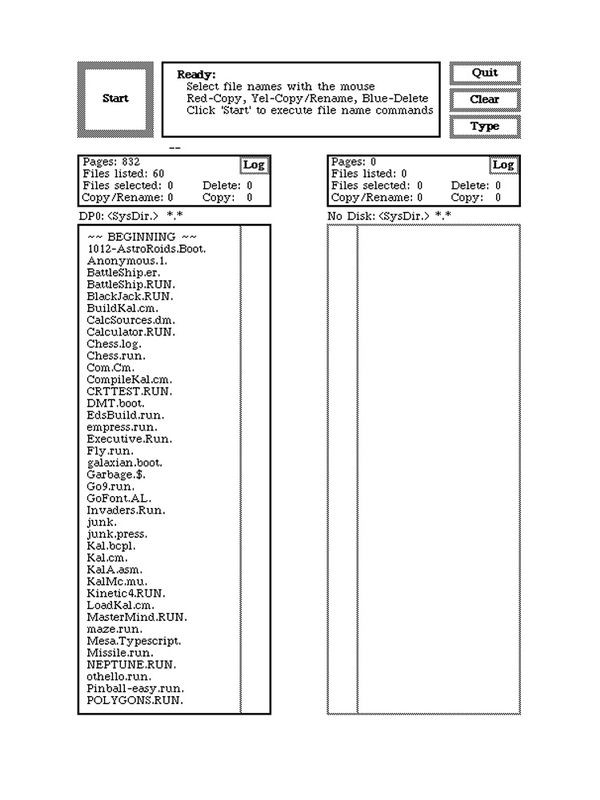
\includegraphics[width=\textwidth]{altoNeptune.png}
            \caption{Alto Neptune Filemanager}
            \label{fig:altoNeptune}
        \end{figure}
        \column{0.3\textwidth}
        \begin{figure}
            \centering
            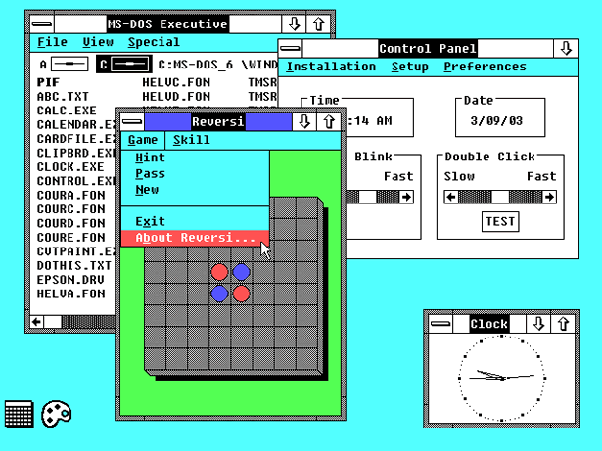
\includegraphics[width=\textwidth]{msdos.png}
            \caption{MS DOS}
            \label{fig:msdos}
        \end{figure}
        \column{0.4\textwidth}
        \begin{figure}
            \centering
            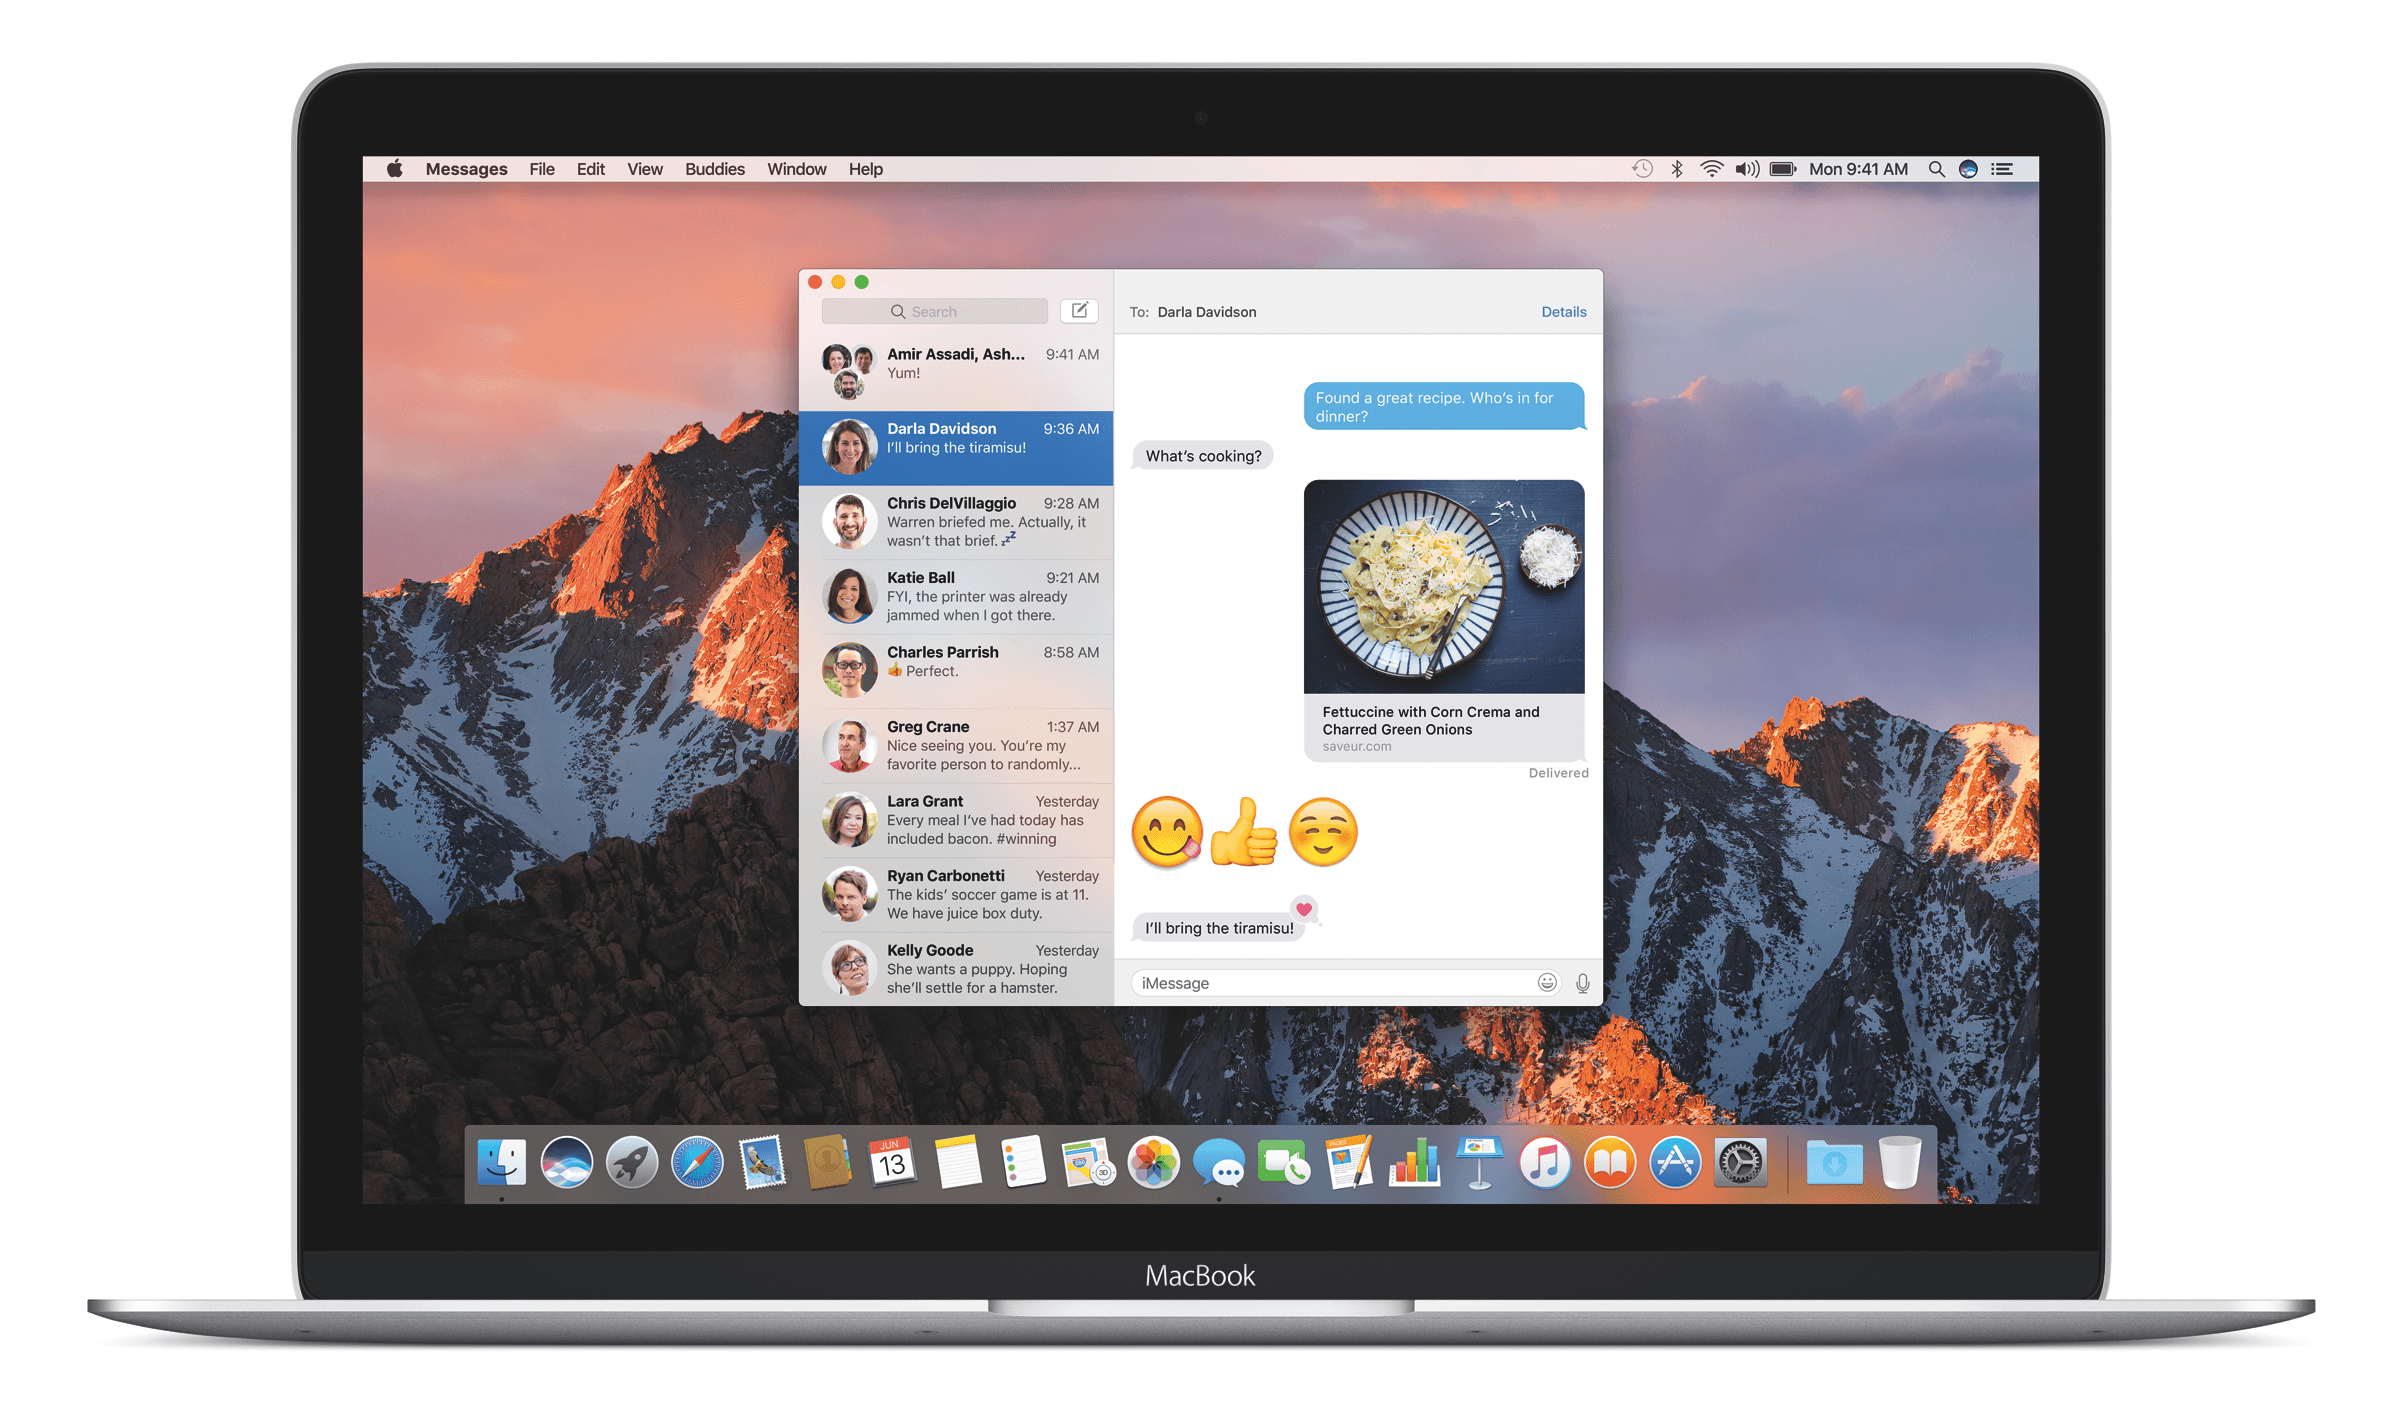
\includegraphics[width=\textwidth]{macos.png}
            \caption{macOS}
            \label{fig:macOS}
        \end{figure}
    \end{columns}
\end{frame}

\begin{frame}{桌面系统}
    事实上,现在我们所说的 Linux 操作系统,本身并不包括桌面环境。Linux 的桌面环境只是 Linux 系统的一个软件,它和内核是不绑定的,两者的开发也不是同步的。给不带界面的 Linux 系统安装上一个桌面环境,你就能看到各种漂亮的窗口,并能用鼠标点击它们了。
\end{frame}

\begin{frame}{GNOME}
    GNOME 的设计目标是为用户提供简单性,易于访问性和可靠性。正因为这些,GNOME 得到了普及。
    
    \begin{figure}
        \centering
        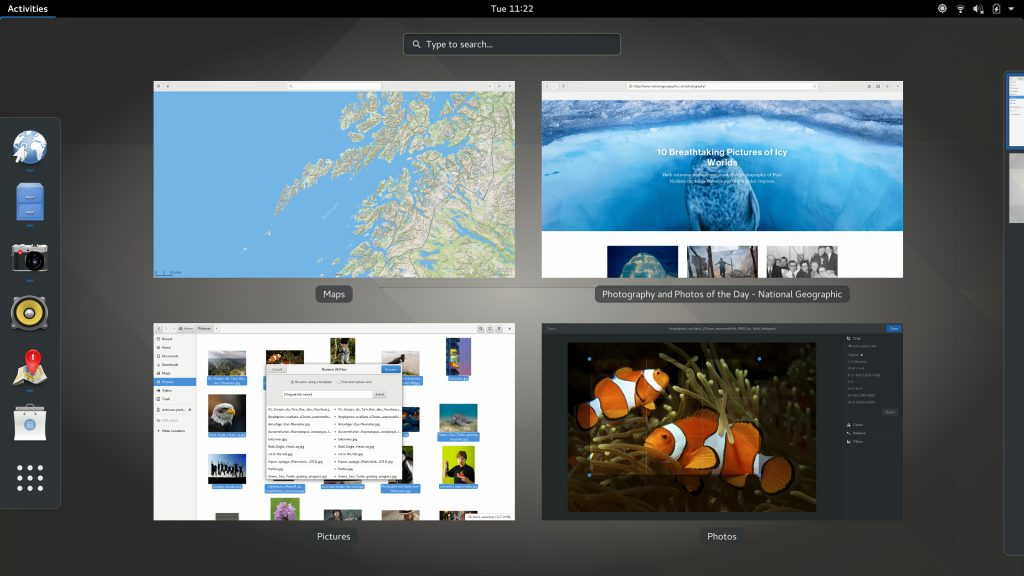
\includegraphics[width=0.8\textwidth]{gnome.png}
        \caption{GNOME}
        \label{fig:gnome}
    \end{figure}
\end{frame}

\begin{frame}{KDE Plasma}
    KDE 软件社区提供的 Plasma Linux 桌面环境是最可定制的图形桌面环境之一。此功能丰富且功能强大的桌面环境还拥有许多小部件。它允许用户自由地添加桌面的控制面板。
    
    \begin{figure}
        \centering
        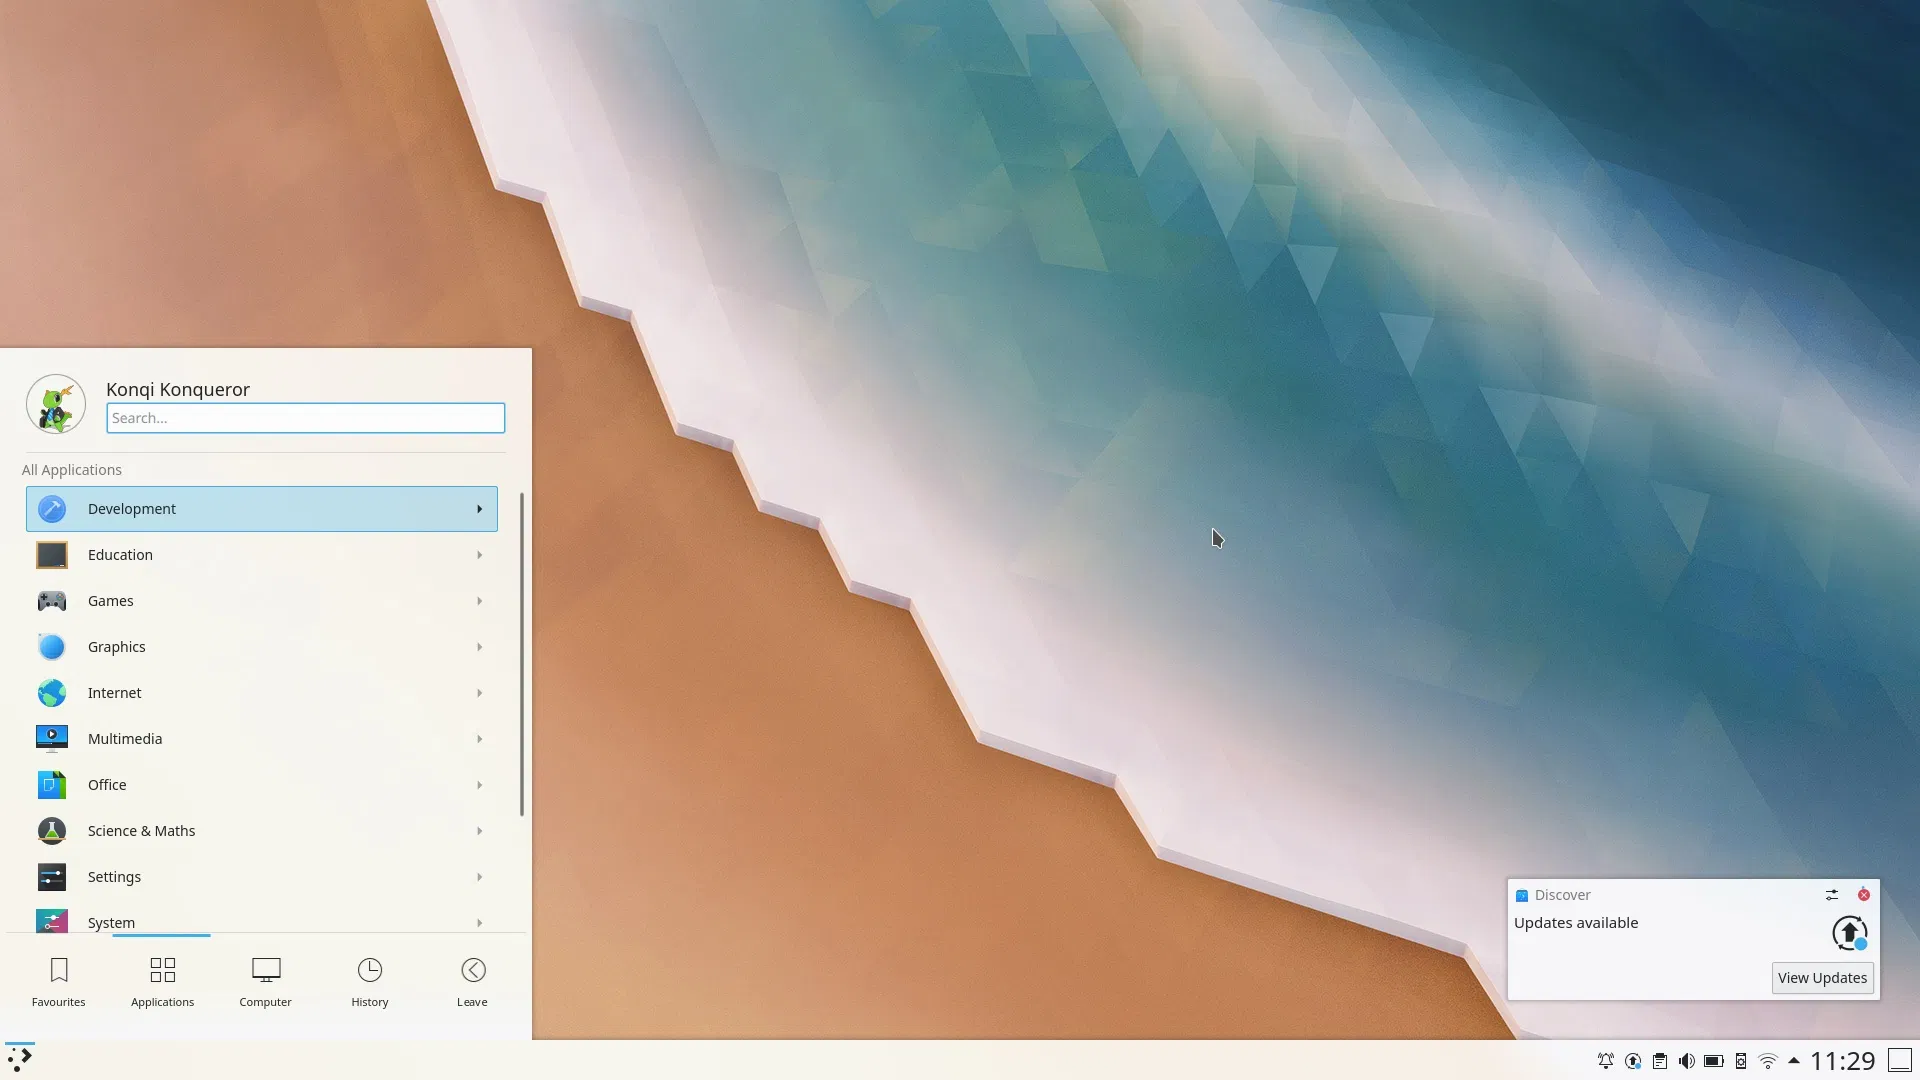
\includegraphics[width=0.75\textwidth]{plasma-5.18.png}
        \caption{KDE Plasma 5.18}
        \label{fig:plasma}
    \end{figure}
\end{frame}

\begin{frame}{Xfce}
    Xfce 是一款快速、轻量,界面美观和对用户友好的桌面环境。
    
    \begin{figure}
        \centering
        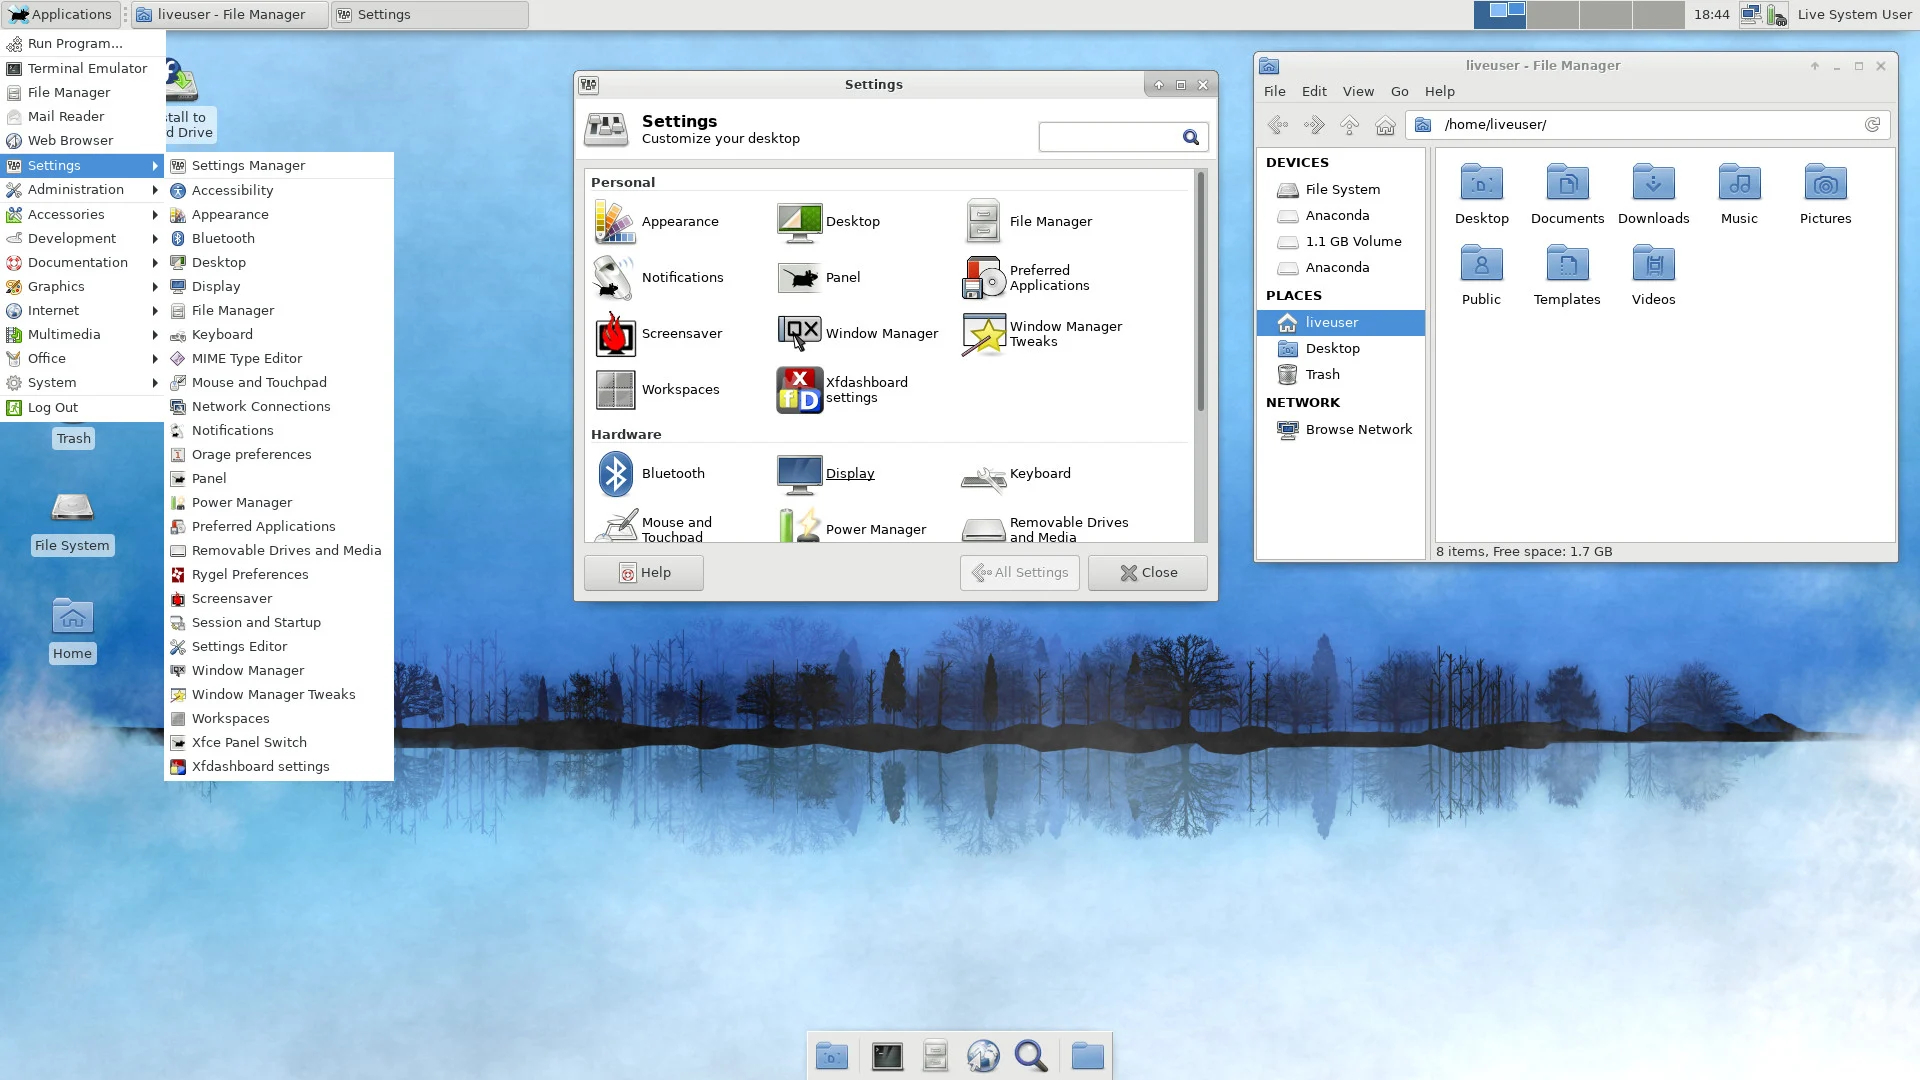
\includegraphics[width=0.8\textwidth]{xfce.png}
        \caption{Fedora 31 Xfce}
        \label{fig:xfce}
    \end{figure}
\end{frame}

\section{个性化桌面系统}

\begin{frame}{个性化桌面系统}
    
\end{frame}
\section{命令行简介}
\begin{frame}{什么是命令行}
    命令行实际上指的就是 shell。shell 其实就是一个程序,它可以接受键盘输入的命令,然后把命令交给系统执行。现在几乎所有的 Linux 发行版都提供了一个叫 bash 的 shell 程序,相当于传统 shell 的增强版。
\end{frame}

\begin{frame}{为什么要用命令行}
\begin{itemize}
    \item 使用命令行很高大上
    \item 使用命令行效率高
    \item 使用命令行可以实现自动化
    \item 使用命令行可以节省资源
\end{itemize}
\end{frame}

\begin{frame}{简单的命令}
    \begin{itemize}
        \item ls: 列出目录的内容
        \item cd: 更改目录
        \item pwd: 查看当前所在的目录
    \end{itemize}
\end{frame}
\section{建站体验}
\end{document}
